% ============================================================
% Unidade 6 — Parte B: erros, observações, exemplos, questões, síntese, respostas
% Fonte única: dossies/u6.md · respostas conferidas em verif/u6.py
% ============================================================
\ErrosComuns

\begin{erro}{Tomar \enquote{$A$ e $B$} por \enquote{só $A$ e $B$}}{6-E1}
\campo{O erro.} Escrever o número de \enquote{$A$ e $B$} direto na região só $A$ e $B$, sem descontar os que estão nos três.
\campo{Por que parece plausível.} \enquote{Os que leem $A$ e $B$} soa como um grupo à parte, separado dos que leem os três.
\campo{Onde quebra.} Numa pesquisa, 10 pessoas leem os jornais $A$ e $B$, e 4 leem os três jornais. Os que leem só $A$ e $B$ são $10-4=6$. Quem escreve 10 na região só $A$ e $B$ conta os 4 duas vezes.
\campo{Como detectar.} O enunciado diz \enquote{só}, \enquote{somente} ou \enquote{mas não $C$}? Se não diz, o número inclui a região central.
\campo{Como corrigir.} Só $A$ e $B$ é $n(A\cap B)-n(A\cap B\cap C)$ (construções 6-H1 e 6-H2).
\campo{Onde aparece.} \exref{ex:u6:streaming} e \exref{ex:u6:clubes}; \qref{u6:uel20}.
\end{erro}

\begin{erro}{Esquecer de devolver os três}{6-E2}
\campo{O erro.} Calcular $n(A\cup B\cup C)$ como $n(A)+n(B)+n(C)$ menos os três pares, e parar aí.
\campo{Por que parece plausível.} Com dois conjuntos, bastava tirar a interseção; parece que basta tirar todas.
\campo{Onde quebra.} Três conjuntos de 10 elementos, com 4 elementos em cada par e 2 nos três: $30-12=18$, mas a reunião tem 20 elementos.
\campo{Como detectar.} Pergunte quantas vezes quem está nos três foi somado e quantas vezes foi tirado.
\campo{Como corrigir.} Some de volta $n(A\cap B\cap C)$ (construção 6-H3).
\campo{Onde aparece.} \exref{ex:u6:streaming}; questões \ref{u6:fme50} e \ref{u6:ufpa24}.
\end{erro}

\begin{erro}{Preencher de fora para dentro}{6-E3}
\campo{O erro.} Calcular só $A$ como $n(A)-n(A\cap B)-n(A\cap C)$.
\campo{Por que parece plausível.} Parece natural tirar de $A$ tudo o que ele divide com os outros.
\campo{Onde quebra.} Com $n(A)=20$, $n(A\cap B)=8$, $n(A\cap C)=6$ e 3 elementos nos três, a conta daria $20-8-6=6$. Mas os 3 do centro foram tirados duas vezes: só $A$ é $20-5-3-3=9$.
\campo{Como detectar.} A região central foi descontada mais de uma vez?
\campo{Como corrigir.} Preencha de dentro para fora (construção 6-H2).
\campo{Onde aparece.} \exref{ex:u6:streaming}; \qref{u6:fme56}.
\end{erro}

\begin{erro}{Confundir \enquote{exatamente dois} com \enquote{pelo menos dois}}{6-E4}
\campo{O erro.} Responder \enquote{exatamente dois} com os que estão em pelo menos dois (ou com a soma dos três pares).
\campo{Por que parece plausível.} \enquote{Estar em dois conjuntos} é verdade também para quem está nos três.
\campo{Onde quebra.} Com pares de 8, 7 e 6 elementos e 3 elementos nos três: exatamente dois são $21-9=12$; pelo menos dois, $12+3=15$. E 21, a soma dos pares, não é nenhum dos dois, porque conta os do centro três vezes.
\campo{Como detectar.} Leia a palavra: \enquote{exatamente} exclui o centro; \enquote{pelo menos} o inclui.
\campo{Como corrigir.} Use $e_2$ e $e_3$ (construção 6-H3, item 2).
\campo{Onde aparece.} \exref{ex:u6:linguas}; questões \ref{u6:ufpe29} e \ref{u6:ufes28}.
\end{erro}

% ------------------------------------------------------------
\Observacoes

\begin{obs}{6-O1}
\textbf{Quando a figura já vem pronta.} Às vezes o enunciado desenha um círculo inteiro dentro de outro, ao modo de Euler. Nesse caso, as regiões que faltam no desenho são regiões vazias. Num diagrama de Venn, com as oito regiões, essas mesmas regiões apareceriam sombreadas: Venn sombreava os compartimentos que uma proposição declara vazios.\src{venn1880}\src{sepDiagrams}
\end{obs}

\begin{obs}{6-O2}
\textbf{E com mais conjuntos?} Para quatro termos, Venn desenhou quatro elipses iguais, que formam dezesseis compartimentos. Para cinco, escreveu que as elipses já não servem na forma simples e propôs uma figura mais complicada; além disso, achava que os diagramas ajudam pouco.\src{venn1880}
\end{obs}

% ------------------------------------------------------------
\Exemplos

\begin{exemplo}{}{1}{autoral}{6-H1, 6-H2, 6-U1, 6-E1, 6-E2, 6-E3}
\label{ex:u6:streaming}
Numa pesquisa com 100 pessoas sobre três serviços de \emph{streaming}, 50 assinam o A, 40 o B e 30 o C; 15 assinam A e B, 10 assinam B e C, 12 assinam A e C, e 5 assinam os três. Preencha as oito regiões. Quantas pessoas assinam pelo menos um serviço? Quantas não assinam nenhum?
\plano De dentro para fora: os três, os \enquote{só dois}, os \enquote{só um}, os de fora.
\resolucao Três: 5. Só A e B: $15-5=10$; só B e C: $10-5=5$; só A e C: $12-5=7$. Só A: $50-10-7-5=28$; só B: $40-10-5-5=20$; só C: $30-7-5-5=13$. Pelo menos um: $28+20+13+10+5+7+5=88$. Nenhum: $100-88=12$.
\begin{center}
\begin{tikzpicture}[scale=0.8]
\draw[thick] (-3.1,-2.75) rectangle (3.1,2.35); \node at (2.8,2.05) {$U$};
\draw[acento,thick] (-0.85,0.45) circle (1.4); \draw[acento,thick] (0.85,0.45) circle (1.4); \draw[acento,thick] (0,-1.0) circle (1.4);
\node at (-2.0,1.75) {A}; \node at (2.0,1.75) {B}; \node at (0,-2.6) {C};
\node at (-1.35,0.85) {28}; \node at (1.35,0.85) {20}; \node at (0,-1.7) {13};
\node at (0,1.05) {10}; \node at (-0.95,-0.55) {7}; \node at (0.95,-0.55) {5}; \node at (0,-0.05) {5};
\node[anchor=south west] at (-3.05,-2.7) {12};
\end{tikzpicture}
\end{center}
\comentario Pela fórmula: $50+40+30-15-10-12+5=88$, o mesmo resultado; sem devolver os 5 dos três, daria 83 (erro 6-E2). Escrever 15 na região só A e B (erro 6-E1), ou calcular só A como $50-15-12$ (erro 6-E3), estragaria todas as contas seguintes.
\end{exemplo}

\begin{exemplo}{}{2}{autoral}{6-H1, 6-H2, 6-U2, 6-E1}
\label{ex:u6:clubes}
Numa escola há três clubes: xadrez (X), música (M) e teatro (T). Participam só do xadrez 8 alunos, só da música 10 e só do teatro 6. Participam de X e M 9 alunos, de M e T 7, de X e T 5, e dos três 3. Sabe-se ainda que 25 alunos não participam do clube de música. Quantos alunos tem a escola?
\plano Completar as regiões \enquote{só dois}; escrever \enquote{não participam de M} como soma de regiões; achar \enquote{nenhum}.
\resolucao Só X e M: $9-3=6$; só M e T: $7-3=4$; só X e T: $5-3=2$. Fora de M estão as regiões só X, só T, só X e T e nenhum: $8+6+2+\text{nenhum}=25$, logo nenhum $=9$. Total: $8+10+6+6+4+2+3+9=48$.
\comentario O dado \enquote{não participam de M} não é o número de nenhum conjunto nem de uma interseção: ele vira uma equação nas regiões.
\end{exemplo}

\begin{exemplo}{}{2}{autoral}{6-H3, 6-E4}
\label{ex:u6:linguas}
Num curso de idiomas, 30 alunos estudam inglês, 25 estudam espanhol e 20 estudam francês. Sabe-se que 12 alunos estudam exatamente duas dessas línguas e 4 estudam as três. Quantos estudam exatamente uma? Quantos estudam pelo menos uma? Quantos estudam pelo menos duas?
\plano Usar $n(I)+n(E)+n(F)=e_1+2e_2+3e_3$, com $e_2=12$ e $e_3=4$.
\resolucao $75=e_1+2\cdot12+3\cdot4$, logo $e_1=39$. Pelo menos uma: $39+12+4=55$. Pelo menos duas: $12+4=16$.
\comentario Não é preciso saber cada par separadamente. Os dados \enquote{exatamente duas} e \enquote{as três} bastam, desde que não se confunda \enquote{exatamente} com \enquote{pelo menos} (erro 6-E4).
\end{exemplo}

\begin{exemplo}{}{2}{autoral}{6-H3, 6-U3}
\label{ex:u6:cafe}
Num grupo de 50 pessoas, 35 tomam café e 30 tomam chá. Qual é o menor número possível de pessoas que tomam as duas bebidas? E o maior?
\plano Chamar de $k$ os que tomam as duas e exigir que nenhuma das quatro regiões fique negativa.
\resolucao Só café: $35-k$; só chá: $30-k$; nenhuma: $50-(35+30-k)=k-15$. Para que nenhuma região seja negativa, $k\ge15$, $k\le35$ e $k\le30$. Logo $k$ vai de 15 a 30.
\comentario O mínimo vem da região \enquote{nenhum}; o máximo, da menor das regiões \enquote{só}. Os dados não dizem quantos tomam as duas bebidas, mas obrigam esse número a ficar entre 15 e 30.
\end{exemplo}

\begin{exemplo}{}{2}{autoral}{6-H1, 6-U4}
\label{ex:u6:elementos}
Determine os conjuntos $A$, $B$ e $C$ sabendo que $A\cup B\cup C=\{1,2,3,4,5,6,7\}$, $A\cap B=\{1,2\}$, $B\cap C=\{1,3\}$, $A\cap C=\{1,4\}$, $A-(B\cup C)=\{5\}$ e $B-(A\cup C)=\{6\}$.
\plano Elemento a elemento: decidir a região de cada um.
\resolucao O 1 está nos três pares, logo nos três conjuntos. O 2 está em $A\cap B$, mas não em $C$ (não está em $B\cap C$); do mesmo modo, o 3 está só em $B$ e $C$, e o 4, só em $A$ e $C$. O 5 está só em $A$, e o 6, só em $B$. O 7 está na reunião, mas não em nenhum dos pares nem nas regiões só $A$ e só $B$: está só em $C$. Logo $A=\{1,2,4,5\}$, $B=\{1,2,3,6\}$ e $C=\{1,3,4,7\}$.
\comentario Cada elemento cai em uma única região; as condições, lidas elemento a elemento, decidem qual.
\end{exemplo}

\begin{exemplo}{}{3}{autoral}{6-H3}
\label{ex:u6:divisiveis}
Quantos números inteiros de 1 a 60 não são divisíveis por 2, nem por 3, nem por 5?
\plano Os conjuntos são definidos por propriedades: $D_2$, $D_3$ e $D_5$. Contar cada um, descobrir quem são as interseções e usar a fórmula de três conjuntos.
\resolucao $n(D_2)=30$, $n(D_3)=20$, $n(D_5)=12$. Ser divisível por 2 e por 3 é ser divisível por 6 (10 números); por 2 e por 5, por 10 (6 números); por 3 e por 5, por 15 (4 números); pelos três, por 30 (2 números). Logo $n(D_2\cup D_3\cup D_5)=30+20+12-10-6-4+2=44$, e os que não são divisíveis por nenhum são $60-44=16$.
\comentario Ninguém informa as interseções: é preciso reconhecê-las como múltiplos de 6, 10, 15 e 30, e contá-las.
\end{exemplo}

% ------------------------------------------------------------
\Questoes

\begin{questao}{1}{FME, exercício 50}{6-H3, 6-E2}\label{u6:fme50}
Sendo $A$, $B$ e $C$ conjuntos finitos, estabeleça uma fórmula para calcular $n(A\cup B\cup C)$.
\resp{$n(A\cup B\cup C)=n(A)+n(B)+n(C)-n(A\cap B)-n(A\cap C)-n(B\cap C)+n(A\cap B\cap C)$; a justificativa deve mostrar que cada elemento da reunião é contado exatamente uma vez.}
\end{questao}

\begin{questao}{1}{FME, exercício 56}{6-H2, 6-U1, 6-E3, 6-E4}\label{u6:fme56}
Uma população consome três marcas de sabão em pó: A, B e C. Feita uma pesquisa de mercado, colheram-se os resultados tabelados abaixo:
\begin{center}
\small
\begin{tabular}{l|cccccccc}
Marca & A & B & C & A e B & B e C & C e A & A, B e C & \begin{tabular}[c]{@{}c@{}}nenhuma\\das três\end{tabular}\\\hline
\begin{tabular}[c]{@{}l@{}}Número de\\consumidores\end{tabular} & 109 & 203 & 162 & 25 & 41 & 28 & 5 & 115
\end{tabular}
\end{center}
Forneça:
\begin{enumerate}[label=\alph*)]
  \item o número de pessoas consultadas;
  \item o número de pessoas que só consomem a marca A;
  \item o número de pessoas que não consomem as marcas A ou C;
  \item o número de pessoas que consomem ao menos duas marcas.
\end{enumerate}
\resp{a) 500;\ b) 61;\ c) 257 (só B e nenhuma: $142+115$);\ d) 84.}
\end{questao}

\begin{questao}{1}{UF-PA via FME, ano não informado}{6-H3, 6-U1, 6-E2}\label{u6:ufpa24}
Feita uma pesquisa entre 100 alunos, do ensino médio, acerca das disciplinas português, geografia e história, constatou-se que 65 gostam de português, 60 gostam de geografia, 50 gostam de história, 35 gostam de português e geografia, 30 gostam de geografia e história, 20 gostam de história e português e 10 gostam dessas três disciplinas. O número de alunos que não gosta de nenhuma dessas disciplinas é:
\begin{multicols}{5}
\begin{enumerate}[label=\alph*)]
  \item 0
  \item 5
  \item 10
  \item 15
  \item 20
\end{enumerate}
\end{multicols}
\resp{a. Gostam de alguma: $175-85+10=100$.}
\end{questao}

\begin{questao}{1}{FEI-SP via FME, ano não informado}{6-H2, 6-U1}\label{u6:fei23}
Em uma comunidade, uma pesquisa a respeito do consumo dos produtos de limpeza A, B e C revelou que 10 consomem os três, 20 consomem os produtos A e C, 40 os produtos B e C, 30 os produtos A e B, 120 o produto C, 160 o produto B, 90 o produto A e 50 não consomem qualquer um dos três produtos. Das pessoas dessa comunidade, $X$ não consomem o produto A. Neste caso:
\begin{multicols}{5}
\begin{enumerate}[label=\alph*)]
  \item $X=250$
  \item $X=370$
  \item $X=180$
  \item $X=200$
  \item $X=330$
\end{enumerate}
\end{multicols}
\resp{a. A comunidade tem 340 pessoas; $340-90=250$.}
\end{questao}

\begin{questao}{2}{UF-PE via FME, ano não informado}{6-H3, 6-E4}\label{u6:ufpe29}
Das companhias que publicam anúncios nos jornais C, D ou F, sabemos que: 30 publicam no C; 25 publicam no D; 30 publicam no F; 10 publicam em C e D; 9 publicam em F e D; 11 publicam em C e F; e 6 publicam em C, D e F. Considerando estas informações, analise as sentenças a seguir.
\begin{itemize}[leftmargin=2.6em,itemsep=0pt]
  \item[0-0)] Onze companhias publicam anúncios em exatamente dois dos jornais.
  \item[1-1)] Dezoito companhias publicam anúncios em pelo menos dois dos jornais.
  \item[2-2)] Quarenta e três companhias publicam anúncios em um único jornal.
  \item[3-3)] Sessenta e uma companhias publicam anúncios em pelo menos um dos três jornais.
  \item[4-4)] Treze companhias publicam anúncios apenas no jornal D.
\end{itemize}
\resp{0-0) F (são 12);\ 1-1) V;\ 2-2) V;\ 3-3) V;\ 4-4) F (são 12).}
\end{questao}

\begin{questao}{2}{FME, exercício 54}{6-H1, 6-H2}\label{u6:fme54}
Considerando os conjuntos $A$, $B$ e $C$, representados abaixo, e sabendo que $n(A\cup B)=24$, $n(A\cap B)=4$, $n(B\cup C)=16$, $n(A-C)=11$ e $n(B-C)=10$, calcule:
\begin{multicols}{2}
\begin{enumerate}[label=\alph*)]
  \item $n(A-B)$
  \item $n(A\cap B\cap C)$
  \item $n(B-(C\cup A))$
  \item $n((A\cap B)-C)$
  \item $n(B-(A\cap B))$
\end{enumerate}
\end{multicols}
\begin{center}
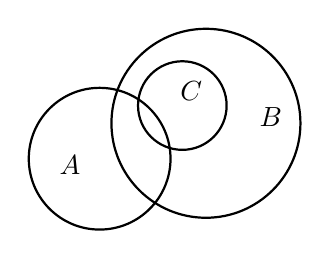
\begin{tikzpicture}[scale=0.75]
\draw[thick] (-0.8,-0.3) circle (1.2); \draw[thick] (1,0.3) circle (1.6); \draw[thick] (0.6,0.6) circle (0.75);
\node at (-1.3,-0.4) {$A$}; \node at (2.1,0.4) {$B$}; \node at (0.75,0.85) {$C$};
\end{tikzpicture}
\end{center}
\resp{a) 8;\ b) 1;\ c) 7;\ d) 3;\ e) 12.}
\end{questao}

\begin{questao}{2}{autoral}{6-H3, 6-U3}\label{u6:natacao}
Numa turma de 40 alunos, 32 fazem natação e 25 fazem judô. Qual é o menor número possível de alunos que fazem os dois esportes? E o maior?
\resp{17 e 25.}
\end{questao}

\begin{questao}{2}{adaptado de U.E. Londrina-PR via FME, ano não informado}{6-H1, 6-U2, 6-E1}\label{u6:uel20}
Um grupo de estudantes resolveu fazer uma pesquisa sobre as preferências dos alunos quanto ao cardápio do Restaurante Universitário. Nove alunos optaram somente por carne de frango, 3 somente por peixes, 7 por carne bovina e frango, 9 por peixe e carne bovina (nesses dois números estão incluídos os que optaram pelos três tipos) e 4 pelos três tipos de carne. Considerando que 20 alunos manifestaram-se vegetarianos, 36 não optaram por carne bovina e 42 não optaram por peixe, assinale a alternativa que apresenta o número de alunos entrevistados.
\begin{multicols}{5}
\begin{enumerate}[label=\alph*)]
  \item 38
  \item 42
  \item 58
  \item 62
  \item 78
\end{enumerate}
\end{multicols}
\resp{c. Só bovina e frango: 3; só peixe e bovina: 5. Fora da bovina: $9+3+\text{(só peixe e frango)}+20=36$, logo só peixe e frango $=4$. Fora do peixe: $9+\text{(só bovina)}+3+20=42$, logo só bovina $=10$. Total: $9+3+10+3+5+4+4+20=58$.}
\end{questao}

\begin{questao}{2}{FGV-SP via FME, ano não informado}{6-H2, 6-H3}\label{u6:fgv36}
Uma pesquisa de mercado sobre determinado eletrodoméstico mostrou que 37\% dos entrevistados preferem a marca X, 40\% preferem a marca Y, 30\% preferem a marca Z, 25\% preferem X e Y, 8\% preferem Y e Z, 3\% preferem X e Z e 1\% prefere as três marcas. Considerando que há os que não preferem nenhuma das três marcas, a porcentagem dos que não preferem nem X nem Y é:
\begin{multicols}{5}
\begin{enumerate}[label=\alph*)]
  \item 20\%
  \item 23\%
  \item 30\%
  \item 42\%
  \item 48\%
\end{enumerate}
\end{multicols}
\resp{e. $n(X\cup Y)=37\%+40\%-25\%=52\%$; nem X nem Y: 48\%.}
\end{questao}

\begin{questao}{2}{UF-ES via FME, ano não informado}{6-H3, 6-U2, 6-E4}\label{u6:ufes28}
Existem, nas cidades brasileiras, 18 milhões de pessoas sem abastecimento público de água potável, 93 milhões sem redes de esgotos sanitários e 14 milhões sem coleta de lixo. Admita que 103 milhões dessas pessoas carecem de pelo menos um desses serviços públicos básicos e que 6 milhões não usufruem de nenhum desses serviços. O número de pessoas, em milhões, que usufruem exatamente um desses serviços é:
\begin{multicols}{5}
\begin{enumerate}[label=\alph*)]
  \item 8
  \item 10
  \item 12
  \item 14
  \item 16
\end{enumerate}
\end{multicols}
\resp{b. Quem usufrui de exatamente um serviço carece de exatamente dois. Com $e_3=6$: $e_1+e_2+6=103$ e $e_1+2e_2+18=125$, logo $e_2=10$.}
\end{questao}

\begin{questao}{2}{UF-PE via FME, ano não informado}{6-H1, 6-H3, 6-U2}\label{u6:ufpe34}
Os alunos de uma turma cursam alguma(s) dentre as disciplinas Matemática, Física e Química. Sabendo que:
\begin{itemize}[leftmargin=1.4em,itemsep=0pt]
  \item o número de alunos que cursam Matemática e Física excede em 5 o número de alunos que cursam as três disciplinas;
  \item existem 7 alunos que cursam Matemática e Química, mas não cursam Física;
  \item existem 6 alunos que cursam Física e Química, mas não cursam Matemática;
  \item o número de alunos que cursam exatamente uma das disciplinas é 150;
  \item o número de alunos que cursam pelo menos uma das três disciplinas é 190.
\end{itemize}
Quantos alunos cursam as três disciplinas?
\resp{22.}
\end{questao}

\begin{questao}{2}{FME, exercício 57}{6-H1, 6-U4}\label{u6:fme57}
Determine os conjuntos $A$, $B$ e $C$ que satisfazem as seguintes seis condições:
\begin{multicols}{2}
\begin{enumerate}[label=\arabic*.ª)]
  \item $A\cup B\cup C=\{z,x,v,u,t,s,r,q,p\}$
  \item $A\cap B=\{r,s\}$
  \item $B\cap C=\{s,x\}$
  \item $C\cap A=\{s,t\}$
  \item $A\cup C=\{p,q,r,s,t,u,v,x\}$
  \item $A\cup B=\{p,q,r,s,t,x,z\}$
\end{enumerate}
\end{multicols}
\resp{$A=\{p,q,r,s,t\}$, $B=\{r,s,x,z\}$, $C=\{s,t,u,v,x\}$.}
\end{questao}

\begin{questao}{3}{UF-MG via FME, ano não informado}{6-H3}\label{u6:ufmg37}
Uma escola realizou uma pesquisa sobre os hábitos alimentares de seus alunos. Alguns resultados dessa pesquisa foram:
\begin{itemize}[leftmargin=1.4em,itemsep=0pt]
  \item 82\% do total de entrevistados gostam de chocolate;
  \item 78\% do total de entrevistados gostam de pizza; e
  \item 75\% do total de entrevistados gostam de batata frita.
\end{itemize}
Então, é correto afirmar que, no total de alunos entrevistados, a porcentagem dos que gostam, ao mesmo tempo, de chocolate, de pizza e de batata frita é, pelo menos, de
\begin{multicols}{4}
\begin{enumerate}[label=\alph*)]
  \item 25\%.
  \item 30\%.
  \item 35\%.
  \item 40\%.
\end{enumerate}
\end{multicols}
\resp{c.}
\end{questao}

\begin{questao}{3}{UF-ES via FME, ano não informado}{6-H1, 6-H3}\label{u6:ufes30}
Em um grupo de 93 torcedores,
\begin{itemize}[leftmargin=1.4em,itemsep=0pt]
  \item todos torcem pelo Flamengo, pelo Cruzeiro ou pelo Palmeiras;
  \item ninguém torce pelo Flamengo e pelo Cruzeiro ao mesmo tempo;
  \item exatamente 12 desses torcedores torcem por dois dos três times;
  \item o número de torcedores que torcem apenas pelo Flamengo é o dobro do número de torcedores que torcem pelo Palmeiras;
  \item pelo menos 4 torcedores torcem apenas pelo Cruzeiro.
\end{itemize}
Com base nessas informações, é correto afirmar que o número máximo possível de torcedores do Palmeiras no grupo é:
\begin{multicols}{5}
\begin{enumerate}[label=\alph*)]
  \item 27
  \item 29
  \item 31
  \item 33
  \item 35
\end{enumerate}
\end{multicols}
\resp{b.}
\end{questao}

\begin{questao}[integradora]{3}{Unicamp-SP via FME, ano não informado}{6-H1, 6-U2}\label{u6:unicamp35}
Três candidatos, A, B e C, concorrem à presidência de um clube. Uma pesquisa apontou que, dos sócios entrevistados, 150 não pretendem votar. Dentre os entrevistados que estão dispostos a participar da eleição, 40 sócios votariam apenas no candidato A, 70 votariam apenas em B e 100 votariam apenas no candidato C. Além disso, 190 disseram que não votariam em A, 110 disseram que não votariam em C e 10 sócios estão na dúvida e podem votar tanto em A como em C, mas não em B. Finalmente, a pesquisa revelou que 10 entrevistados votariam em qualquer candidato. Com base nesses dados, pergunta-se:
\begin{enumerate}[label=\alph*)]
  \item Quantos sócios entrevistados estão em dúvida entre votar em B ou em C, mas não votariam em A? Dentre os sócios consultados que pretendem participar da eleição, quantos não votariam em B?
  \item Quantos sócios participaram da pesquisa? Suponha que a pesquisa represente fielmente as intenções de voto de todos os sócios do clube. Escolhendo um sócio ao acaso, qual a probabilidade de que ele vá participar da eleição mas ainda não tenha se decidido por um único candidato?
\end{enumerate}
(Sugestão: utilize o diagrama de Venn.)
\resp{a) 20; 150;\ b) 400; $\frac{40}{400}=\frac{1}{10}$ (probabilidade = casos favoráveis $\div$ total).}
\end{questao}

\subsubsection*{Mais questões de vestibular}
Questões de vestibular sobre o assunto da unidade que ficaram fora da sequência acima, em ordem de nível. As respostas estão no fim da unidade, com as demais.

\begin{questao}{1}{U.E. Londrina-PR via FME, ano não informado}{6-H3, 6-U1}\label{u6:uel25}
Num dado momento, três canais de TV tinham, em sua programação, novelas em seus horários nobres: a novela A no canal A, a novela B no canal B e a novela C no canal C. Numa pesquisa com 3\,000 pessoas, perguntou-se quais novelas agradavam. A tabela a seguir indica o número de telespectadores que designaram as novelas como agradáveis.
\begin{center}
\small
\begin{tabular}{l|ccccccc}
Novelas & A & B & C & A e B & A e C & B e C & A, B e C\\\hline
Número de espectadores & 1\,450 & 1\,150 & 900 & 350 & 400 & 300 & 100
\end{tabular}
\end{center}
Quantos telespectadores entrevistados não acham agradável nenhuma das três novelas?
\begin{multicols}{3}
\begin{enumerate}[label=\alph*)]
  \item 300 telespectadores.
  \item 370 telespectadores.
  \item 450 telespectadores.
  \item 470 telespectadores.
  \item 500 telespectadores.
\end{enumerate}
\end{multicols}
\resp{c.}
\end{questao}

\begin{questao}{2}{UF-PA via FME, ano não informado}{6-H3}\label{u6:ufpa26}
Um professor de Matemática, ao lecionar Teoria dos Conjuntos em uma certa turma, realizou uma pesquisa sobre as preferências clubísticas de seus $n$ alunos, tendo chegado ao seguinte resultado:
\begin{itemize}[leftmargin=1.4em,itemsep=0pt]
  \item 23 alunos torcem pelo Paysandu Sport Club;
  \item 23 alunos torcem pelo Clube do Remo;
  \item 15 alunos torcem pelo Clube de Regatas Vasco da Gama;
  \item 6 alunos torcem pelo Paysandu e pelo Vasco;
  \item 5 alunos torcem pelo Vasco e pelo Remo.
\end{itemize}
Se designarmos por $A$ o conjunto dos torcedores do Paysandu, por $B$ o conjunto dos torcedores do Remo e por $C$ o conjunto dos torcedores do Vasco, todos da referida turma, teremos, evidentemente, $A\cap B=\varnothing$. Concluímos que o número $n$ de alunos desta turma é
\begin{multicols}{5}
\begin{enumerate}[label=\alph*)]
  \item 49.
  \item 50.
  \item 47.
  \item 45.
  \item 46.
\end{enumerate}
\end{multicols}
\resp{b. Como $A\cap B=\varnothing$, também $A\cap B\cap C=\varnothing$: $23+23+15-6-5=50$ (supondo, como o enunciado sugere, que todos torcem por algum dos três).}
\end{questao}

\begin{questao}{2}{UF-PE via FME, ano não informado}{6-H3}\label{u6:ufpe31}
Em uma pesquisa com os 60 alunos de uma turma do ensino médio sobre a preferência deles com respeito às disciplinas Matemática, Física e Química, foi constatado que:
\begin{itemize}[leftmargin=1.4em,itemsep=0pt]
  \item 14 alunos gostam de exatamente duas das três disciplinas;
  \item 20 alunos gostam das três disciplinas;
  \item 10 alunos não gostam de nenhuma das três disciplinas.
\end{itemize}
Quantos alunos gostam de exatamente uma das três disciplinas?
\begin{multicols}{5}
\begin{enumerate}[label=\alph*)]
  \item 18
  \item 17
  \item 16
  \item 15
  \item 14
\end{enumerate}
\end{multicols}
\resp{c.}
\end{questao}

\begin{questao}{2}{Udesc-SC via FME, ano não informado}{6-H1, 6-H2}\label{u6:udesc22}
\textbf{O que os brasileiros andam lendo?} O brasileiro lê, em média, 4,7 livros por ano. Este é um dos principais resultados da pesquisa \emph{Retratos da Leitura no Brasil}, encomendada pelo Instituto Pró-Livro ao Ibope Inteligência, que também pesquisou o comportamento do leitor brasileiro, as preferências e as motivações dos leitores, bem como os canais e a forma de acesso aos livros. (Fonte: Associação Brasileira de Encadernação e Restauro, adapt.)

Supõe-se que em uma pesquisa envolvendo 660 pessoas, cujo objetivo era verificar o que elas estão lendo, obtiveram-se os seguintes resultados: 100 pessoas leem somente revistas, 300 pessoas leem somente livros e 150 pessoas leem somente jornais. Supõe-se ainda que, dessas 660 pessoas, 80 leem livros e revistas, 50 leem jornais e revistas, 60 leem livros e jornais e 40 leem revistas, jornais e livros. Em relação ao resultado dessa pesquisa, são feitas as seguintes afirmações:
\begin{enumerate}[label=\Roman*.]
  \item Apenas 40 pessoas leem pelo menos um dos três meios de comunicação citados.
  \item Quarenta pessoas leem somente revistas e livros, e não leem jornais.
  \item Apenas 440 pessoas leem revistas ou livros.
\end{enumerate}
Assinale a alternativa correta.
\begin{enumerate}[label=\alph*)]
  \item Somente as afirmativas I e III são verdadeiras.
  \item Somente as afirmativas I e II são verdadeiras.
  \item Somente as afirmativas I, II e III são verdadeiras.
  \item Somente a afirmativa II é verdadeira.
  \item Somente a afirmativa I é verdadeira.
\end{enumerate}
\resp{d.}
\end{questao}

\begin{questao}{2}{UF-PI via FME, ano não informado}{6-H2, 6-H3}\label{u6:ufpi27}
O diretor de uma tradicional escola da cidade de Teresina resolveu fazer uma pesquisa de opinião junto aos seus 590 alunos do Ensino Médio sobre as políticas públicas de acesso ao Ensino Superior. No questionário, perguntava-se sobre a aprovação de: Cotas, Bolsas e Enem, como modelo de exame vestibular. As respostas dos alunos foram sintetizadas na tabela abaixo:
\begin{center}
\small
\begin{tabular}{l|ccccccc}
Política pública & Cotas & Bolsas & Enem & \begin{tabular}[c]{@{}c@{}}Cotas e\\Bolsas\end{tabular} & \begin{tabular}[c]{@{}c@{}}Bolsas e\\Enem\end{tabular} & \begin{tabular}[c]{@{}c@{}}Cotas e\\Enem\end{tabular} & \begin{tabular}[c]{@{}c@{}}Cotas, Bolsas\\e Enem\end{tabular}\\\hline
Número de aprovações & 226 & 147 & 418 & 53 & 85 & 116 & 44
\end{tabular}
\end{center}
Sobre a pesquisa e a tabela anterior, é correto afirmar que
\begin{enumerate}[label=\alph*)]
  \item a quantidade de alunos que não opinaram por nenhuma das três políticas é 12.
  \item a quantidade de alunos que aprovam apenas uma política pública é 415.
  \item a quantidade de alunos que aprovam mais de uma política é 167.
  \item a quantidade de alunos que aprovam as três políticas é 45.
  \item há mais alunos que aprovam cotas do que alunos que aprovam somente o Enem.
\end{enumerate}
\resp{b.}
\end{questao}

\begin{questao}{2}{adaptado de U.F. Uberlândia-MG via FME, ano não informado}{6-H1, 6-U2, 6-E1}\label{u6:ufu33}
De uma escola de Uberlândia, partiu uma excursão para Caldas Novas com 40 alunos. Ao chegar em Caldas Novas, 2 alunos adoeceram e não frequentaram as piscinas. Todos os demais alunos frequentaram as piscinas, sendo 20 pela manhã e à tarde (incluídos os que foram também à noite), 12 somente pela manhã, 3 somente à noite e 8 pela manhã, à tarde e à noite. Se ninguém frequentou as piscinas somente no período da tarde, quantos alunos frequentaram as piscinas à noite?
\begin{multicols}{4}
\begin{enumerate}[label=\alph*)]
  \item 16
  \item 12
  \item 14
  \item 18
\end{enumerate}
\end{multicols}
\resp{c.}
\end{questao}

\begin{questao}{3}{UF-PE via FME, ano não informado}{6-H1}\label{u6:ufpe19}
Os 200 estudantes de uma escola que praticam esportes escolhem duas dentre as modalidades seguintes: futebol, handebol, basquete e futebol de salão. Entretanto, nenhum estudante da escola escolheu futebol e basquete ou handebol e futebol de salão. Sabendo que 65\% dos alunos escolheram futebol, 60\% escolheram futebol de salão, 35\% escolheram basquete e 25\% dos jogadores de handebol também jogam basquete, quantos são os alunos da escola que jogam futebol e futebol de salão?
\resp{70.}
\end{questao}

\begin{sintese}
\textbf{Ao fim desta unidade, você deveria saber:}
\begin{itemize}[leftmargin=1.4em,itemsep=1pt]
  \item desenhar as oito regiões de três conjuntos e preenchê-las de dentro para fora;
  \item calcular $n(A\cup B\cup C)$ e explicar por que os que estão nos três são devolvidos;
  \item distinguir \enquote{$A$ e $B$} de \enquote{só $A$ e $B$}, e \enquote{exatamente dois} de \enquote{pelo menos dois};
  \item transformar dados indiretos em equações nas regiões;
  \item achar o menor e o maior valor que os dados permitem, exigindo que nenhuma região seja negativa;
  \item determinar conjuntos elemento a elemento.
\end{itemize}
\smallskip\noindent\textbf{Responda com suas palavras, sem consultar.} Depois, confira com a caixa \emph{Para lembrar} (p.~\pageref{lembrar-u6}) e com a seção indicada.
\begin{enumerate}[label=\arabic*.,leftmargin=1.4em]
  \perguntasintese{Por que se desenham as oito regiões, mesmo as que podem estar vazias? \ondever{construção 6-H1}}
  \perguntasintese{Por que, na fórmula de três conjuntos, a interseção dos três é somada de volta? \ondever{construção 6-H3}}
  \perguntasintese{Num enunciado, como você reconhece que os dados só limitam a resposta, e o que faz então? \ondever{Onde é usado?}}
  \perguntasintese{Qual erro você cometeria ao escrever o número de \enquote{$A$ e $B$} direto na região só $A$ e $B$? Como evitá-lo? \ondever{Erros comuns}}
\end{enumerate}
\end{sintese}

% ------------------------------------------------------------
\Respostas
{\small\resposta{S}{Síntese de domínio: confira com a caixa \emph{Para lembrar} (p.~\pageref{lembrar-u6}) e com a seção indicada em cada pergunta.}}
